% Канонический TikZ-рисунок варианта 14. Править только здесь.
\long\def\figStereoV14{%
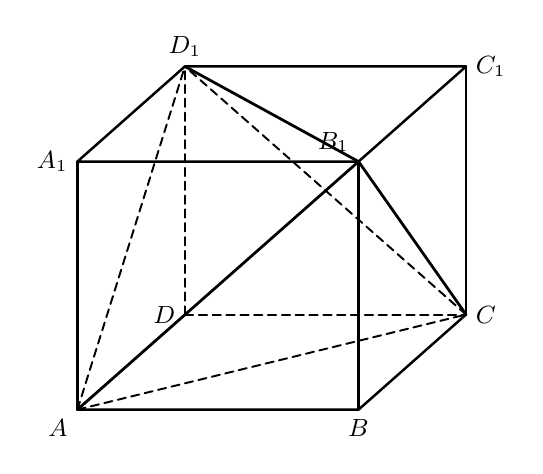
\begin{tikzpicture}[
    scale=1.05,
    line cap=round,
    line join=round,
    edge/.style={
        line width=0.9pt
    },
    hidden/.style={
        line width=0.7pt,
        dashed,
        dash pattern=on 3pt off 2pt
    },
    section/.style={
        line width=1pt
    },
    every node/.style={
        font=\small
    }
]

% =================================================
% Вершины параллелепипеда
% =================================================

% Нижнее основание ABCD
\coordinate (A) at (0,0);
\coordinate (B) at (3.4,0);
\coordinate (C) at (4.7,1.15);
\coordinate (D) at (1.3,1.15);

% Верхнее основание A_1B_1C_1D_1
\coordinate (A1) at (0,3);
\coordinate (B1) at (3.4,3);
\coordinate (C1) at (4.7,4.15);
\coordinate (D1) at (1.3,4.15);

% =================================================
% Скрытые рёбра параллелепипеда
% =================================================

\draw[hidden] (A)--(D);
\draw[hidden] (D)--(C);
\draw[hidden] (D)--(D1);

% =================================================
% Видимые рёбра параллелепипеда
% =================================================

\draw[edge] (A)--(B)--(C);
\draw[edge] (A)--(A1);
\draw[edge] (B)--(B1);
\draw[edge] (C)--(C1);

\draw[edge]
    (A1)--(B1)--(C1)--(D1)--cycle;

% =================================================
% Рёбра пирамиды ACB_1D_1
% =================================================

% Ребро AC лежит в нижнем основании
\draw[hidden] (A)--(C);

% Рёбра, соединяющие нижние и верхние вершины
\draw[section] (A)--(B1);
\draw[hidden]  (A)--(D1);

\draw[section] (C)--(B1);
\draw[hidden] (C)--(D1);

% Ребро B_1D_1 лежит в верхнем основании
\draw[section] (B1)--(D1);

% =================================================
% Подписи
% =================================================

\node[below left]  at (A)  {$A$};
\node[below]       at (B)  {$B$};
\node[right]       at (C)  {$C$};
\node[left]        at (D)  {$D$};

\node[left]        at (A1) {$A_1$};
\node[above left]  at (B1) {$B_1$};
\node[right]       at (C1) {$C_1$};
\node[above]       at (D1) {$D_1$};

\end{tikzpicture}
}
